\section{Vertical Shifting}

Very similar to the horizontal position change, the vertical position change
merely requires the transformation matrix to be shifted row-wise as opposed
to
column-wise.
\[
  \underbrace{
    \begin{bmatrix}
      1&0&0\\
      0&1&0\\
      0&0&1\\
    \end{bmatrix}
  }_{\text{Identity Matrix}}
  \implies
  \underbrace{
    \begin{bmatrix}
      0&0&1\\
      1&0&0\\
      0&1&0\\
    \end{bmatrix}
  }_{\text{Transformation
  Matrix}}
\]
\[ 
  \begin{bmatrix}
    0&0&1\\
    1&0&0\\
    0&1&0\\
  \end{bmatrix}
  \cdot
  \begin{bmatrix}
    a&b&c\\
    d&e&f\\
    g&h&i\\
  \end{bmatrix}
  =
  \underbrace{
    \begin{bmatrix}
    g&h&i\\
    a&b&c\\
    d&e&f\\
    \end{bmatrix}
  }_{\text{The
    vertically
    shifted
  matrix}}
\]

\begin{figure}[ht]
  \centering
  \begin{subfigure}{\textwidth}
    \centering
    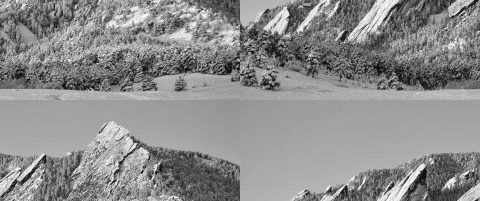
\includegraphics[scale=0.7]{./img/vhsg1.png}
    \caption{Photo 1 - Vertical and
    Horizontal Shift}
    \label{fig:p1vg}
  \end{subfigure}
  \begin{subfigure}{\textwidth}
    \centering
    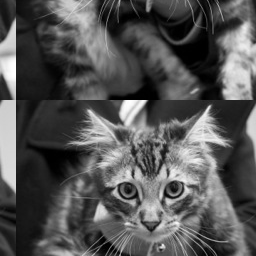
\includegraphics[scale=0.7]{./img/vhsg2.png}
    \caption{Photo
      2
      -
      Vertital
      and
      Horizontal
    Shift}
    \label{fig:p2vg}
  \end{subfigure}
  \caption{Vertically
    Shifted
  Images}
  \label{fig:vs_images}
\end{figure}
